\documentclass{matmex-diploma-custom}



\begin{document}
% Год, город, название университета и факультета предопределены,
% но можно и поменять.
% Если англоязычная титульная страница не нужна, то ее можно просто удалить.
\filltitle{ru}{
 university = {Правительство Российской Федерации\\Федеральное государственное бюджетное образовательное учреждение высшего профессионального образования\\
«Санкт-Петербургский государственный университет»},
	faculty = {\hfill},
    chair              = {Кафедра Системного Программирования},
    title              = {Скрытые Марковские модели переменного порядка для анализа
данных ChIP-seq},
    % Здесь указывается тип работы. Возможные значения:
    %   coursework - Курсовая работа
    %   diploma - Диплом специалиста
    %   master - Диплом магистра
    %   bachelor - Диплом бакалавра
    type               = {bachelor},
    position           = {студента},
    group              = 444,
    author             = {Атаманова Анна Михайловна},
    supervisorPosition = {д.\,ф.-м.\,н., профессор},
    supervisor         = {Терехов А.\,Н.},
    reviewerPosition   = {},
    reviewer           = {Лебедев С.\,A.},
    chairHeadPosition  = {д.\,ф.-м.\,н., профессор},
    chairHead          = {Терехов А.\,Н.},
%   university         = {Санкт-Петербургский Государственный Университет},
%   faculty            = {Математико-механический факультет},
%    city               = {Санкт-Петербург},
%   year               = {2015}
}
\filltitle{en}{
	type 			  = {bachelor},
	faculty 			  = {\hfill},
    chair              = {Chair of Software Engineering},
    title              = {Variable-length hidden Markov models for ChIP-seq data analysis},
    author             = {Anna Atamanova},
    supervisorPosition = {professor},
    supervisor         = {Andrey Terekhov},
    reviewerPosition   = {},
    reviewer           = {Sergei },
    chairHeadPosition  = {professor},
    chairHead          = {Andrey Terekhov},
}
\maketitle
\tableofcontents
% У введения нет номера главы
\section*{Введение}
\subsection*{Предметная область}
Наш организм состоит из огромного количества клеток. Которые находятся в непрерывном движении. Вся жизнь наша заключается в их функционировании. Одна из интереснейших частей клетки --- это ее память, ДНК (дезоксирибонуклеиновая кислота), которая хранит в себе просто неимоверное количество информации, в том числе <<рецепты>> построения необходимых веществ. Своеобразным строительным материалом клетки является белок. Белок также выполняет структурные, сигнальные, механические и другие функции. Соединения ДНК с конкретным белком могут играть роль в структуре ДНК, во внутренних механизмах управления клетки. Поэтому изучение ДНК-белковых взаимодействий крайне важно и актуально.

Однако перед самим изучением взаимодействий, необходимо обнаружить/распознать места, где они случились.

Данная работа посвящена изучению нахождения позиций связывания конкретного белка и ДНК, то есть нахождения позиций ДНК-белковых взаимодействий при заранее выбранном белке.

\subsection*{ChIP-seq}
ChIP-seq (chromatin immunoprecipitation sequencing) --- биологический эксперимент, позволяющий получить информацию о наличие или отсутствии
взаимодействия ДНК с заданным белком вдоль всего генома.

Схематично, эксперимент на тысячах одинаковых клеток (при заранее выбранном изучаемом белке) проводит следующие шаги:
\begin{enumerate}
\item приклеивает все обнаруженные белки к ДНК;
\item расщепляет ДНК на фрагменты;
\item вылавливает фрагменты, связанные с исследуемым белком (с помощью специфичного к исследуемому белку антитела);
\item считывает фрагменты (специальный прибор -- секвенатор считывает только концы фрагментов, т.к. целый фрагмент слишком велик; cчитанный кусок фрагмента называется прочтением или ридом; cчитается, что в итоге каждый фрагмент с высокой вероятностью считан несколько раз).
\end{enumerate} 

Далее для каждого полученного рида ищется соответствующий
ему участок последовательности генома (рис.~\ref{fig:chip-seq}). Обычно
риды, которым может соответствовать более одного участка в геноме,
исключают из рассмотрения.

\begin{figure}[h]
  \centering

\begin{Verbatim}[commandchars=\\\{\}]
          CAAAAGACAAATAGTGATGTCACCAATCGAGC
          --------------------------------
               GACA ATA     GTCA  AATC
              AGAC   TAGTG TGTC
               GACA   AGTG TGTCA   ATCG

          00001100001110000110000011000000
\end{Verbatim}
  \caption{Схематическое изображение выравнивания прочтений секвенатора (под чертой)
    на известную последовательность генома (над чертой).}
  \label{fig:chip-seq}
\end{figure}

Результаты эксперимента представляют в виде массива длины генома, в позиции которого стоит 1, если в соответствующей позиции генома начиналось хотя бы одно прочтение
и 0 в обратном случае.

Однако, белок мог находиться не в самом начале фрагмента, и, кроме того, соединение белка с ДНК происходит не точечно, а на некотором участке ДНК.
Поэтому, для дальнейшего анализа, полученный массив разбивается на отрезки заранее выбранной длины, называемые окнами (обычно 200 пн (пар нуклеотидов)). Значение в окне определяется как сумма единиц в нем. 

Эксперимент ChIP-seq (как и большинство биологических
экспериментов) не исключает наличие ошибок в результатах. Недостаточная специфичность антитела, наличие ошибок секвенирования, нестабильность положения белка на ДНК приводят к возникновению сигнала, не
зависящего от наличия взаимосвязи.
Поэтому, для дальнейшего анализа результатов эксперимента, требуется построение вероятностной модели, способной отделять ошибки, а также 
выявлять зависимости соединений и, по возможности, описывать их структуру.

Большинство существующих моделей (\cite{Zhang2008}, \cite{Spyrou2009}) для данных
хроматин-иммунопреципитации основано на аппарате скрытых Марковских моделей (СММ) \cite{Rabiner1989}
первого порядка с Пуассоновскими испусканиями. Использование распределения
Пуассона для покрытия опирается на предположение о том, что в каждой
позиции генома в среднем начинается одинаковое количество прочтений.
Марковский процесс, как правило, имеет два состояния <<$1$>> --- сигнал есть и <<$0$>> --- сигнала нет. Первый порядок модели означает, что состояние некоторого окна зависит только от состояния его прямого предшественника.
Использование моделей первого порядка объясняется тем, что количество параметров
модели, а также сложность её обучения и использования экспоненциально зависят от
порядка. Так, СММ порядка $ m $ для каждой цепочки из $ m $ состояний содержит распределение на следующее состояние ($ 2^m $ вероятностных распределений). В связи с этим, неправильный выбор $ m $ в обучении сильно усложняет модель и способствует ее переобучению. 

Скрытые Марковские модели переменного порядка избегают такого эффекта, т.к. они не фиксируют длину строки, порождающей следующее состояние, и стараются ее уменьшить.

\section{Постановка задачи}
Целью данной дипломной работы является построение скрытой Марковской модели переменного
порядка для анализа данных ChIP-seq.

Для достижения цели были определены следующие задачи:
\begin{enumerate}
\item
реализация скрытой Марковской модели
переменного порядка;
\item
анализ эффективности работы модели на синтетических
данных;
\item
применение к данным ChIP-seq, сравнение с более простыми моделями (СММ
первого порядка).
\end{enumerate}


\section{Обзор существующих решений}
Марковские модели переменного порядка (не скрытые) обучаются путем построения контекстного дерева переходов \cite{Buhlmann1999}. Скрытые Марковские модели фиксированного порядка обучаемы алгоритмом Баума-Велша \cite{Rabiner1989}.
Совмещение этих двух идей дает возможность обучить скрытые Марковские модели переменного порядка (СММПП). Такой подход обучения был предложен в \cite{Wang2006}. 

В данной работе алгоритмом обучения СММПП был выбран модифицированный под поставленную задачу алгоритм  из \cite{Wang2006}. Он был дополнен недостающей информацией об обучении контекстных деревьев из статей \cite{Buhlmann1999}, \cite{Dumont2014}.
Модификация заключается в следующем: наблюдения итоговой модели будут порождаться из соответствующих состояний, т.е. распределение значений для каждого окна задается скрытым состоянием, которое определяет, была ли там взаимосвязь с белком или нет. В работе \cite{Wang2006} такие распределения определялись всем контекстом. 

\subsection{Основные понятия и определения}

Путь 
$ S = \{0, 1\} $ --- множество состояний (в рамках рассматриваемой задачи, 1 означает наличие связи, 0 --- ее отсутствие), 
$X_0, X_1, \ldots $ --- последовательность случайных величин (дискретный случайный процесс), значения которых лежат в S, а
$x_0, x_1, \ldots$ - некоторая реализация случайных величин $X_0, X_1, \ldots $.

\begin{definition} $ \{X_{i}\}_{i \in Z_{+}}$ называется \emph{Марковским процессом порядка $ m $}, если  
\begin{align*}
&\forall t, t'\in N, \;t, t' \geq m,\; \forall \overrightarrow{x} \in S^{t+1}
\\&P(X_{t} = x_{t}|X_{t-1}=x_{t-1},X_{t-2}=x_{t-2}, \ldots ,X_{0}=x_{0}) 
\\&=P(X_{t} = x_{t}|X_{t-1}=x_{t-1},X_{t-2}=x_{t-2}, \ldots ,X_{t-m}=x_{t-m})
\\&=P(X_{t'} = x_{t}|X_{t'-1}=x_{t-1},X_{t'-2}=x_{t-2}, \ldots ,X_{t'-m}=x_{t-m})
\\&=P(X_{t'} = x_{t}|X_{t'-1}=x_{t-1},X_{t'-2}=x_{t-2}, \ldots ,X_{0}=x_{0}) 
\end{align*}
\label{MP}
\end{definition}
Далее, для Марковских процессов, вероятности вида  
$$P(X_{t'} = x_{t}|X_{t'-1}=x_{t-1},X_{t'-2}=x_{t-2}, \ldots ,X_{t'-m}=x_{t-m})$$ где $t'\geq m$, 
\\будем записывать как $P(x_{t} |x_{t-1}\ldots x_{t-m})$ (запись корректна, в силу независимости такой вероятности от $t'$).

Для удобства будем считать, что наш процесс растет справа налево  
$$\ldots x_{t},~ x_{t-1},~ x_{t-2} \ldots$$
Так,  если цепь $\ldots x_{t}, x_{t-1}, x_{t-2} \ldots$ была порождена процессом порядка $2$,
то $$P(x_{t}| x_{t-1},x_{t-2}\ldots) = P(x_{t}|x_{t-1},x_{t-2})$$

\begin{definition} \emph{Марковская модель порядка $ m $} --- это вероятностная модель, описывающая марковский процесс порядка $m$. Параметрами модели являются множество переходов  $ A = \{a(q; x^{m})\}_{q \in S, x^{m} \in S^{m}}$, где $a(q; x^{m}) = P(q|x^{m})$, и начальное распределение $\pi = \pi(x^m)_{x^m \in S^m}$, где $\pi(x^m) = P(X_{0:m}=x^m)$.
\end{definition}

\textit{Контекстом} состояния $ x_{t} $  будем называть любой префикс строки  $x_{t-1}, x_{t-2} \ldots$. 

\begin{definition}
\textit{Контекстное дерево} --- это дерево, в котором каждая внутренняя вершина имеет $ |S| $ ребер, соответствующих состояниям из $S$, и метку, которая является конкатенацией метки на ее родителе и метки ребра от него. Метка в корне --- пустая строка.
\end{definition}
Контексты, соответствующие листьям контекстного дерева, будем называть \textit{главными контекстами} (иногда, когда речь будет идти только о листьях, слово <<главные>> будем опускать).

Множество переходов для Марковского процесса порядка $ m $ можно определить, как контекстное дерево глубины $ m+1 $, каждый лист которого содержит распределение $P(.~|~w)$, где $ w $ --- метка на листе.

Для того, чтобы по дереву определить распределение на следующем состоянии $ X_{t} $, достаточно из корня спуститься по ветке, вершины которой соответствуют контекстам этого состояния, $(x_{t-1}),\; (x_{t-1}x_{t-2}), \ldots$ . Лист на конце ветки и будет задавать распределение $ X_{t} $.


\begin{remark}
Метки на листьях контекстного дерева определяют все дерево.
\end{remark}

На рисунке \ref{ris:context_trie} изображен пример контекстного дерева для Марковского процесса порядка $ 2 $ (серым подкрашены листья, ниже прямоугольниками обозначены распределения переходов).
\begin{figure}[h!]\centering
\begin{minipage}[b]{0.49 \textwidth}
	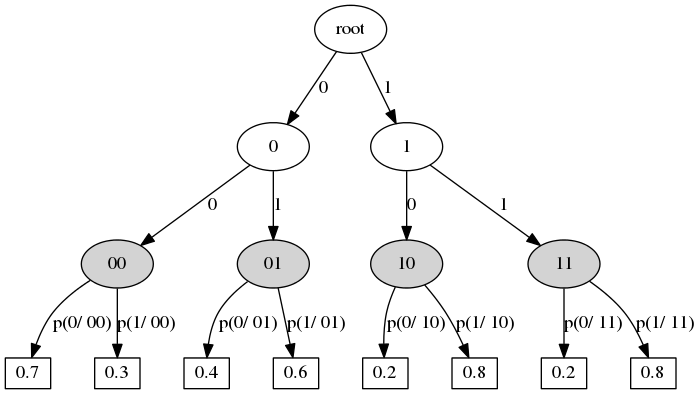
\includegraphics[scale=0.38]{img/Context_trie.pdf}
	\centering
	\caption{ Контекстное дерево переходов Марковского процесса порядка 2 }
	\label{ris:context_trie}
	
\end{minipage}
\hfil \hfil
\begin{minipage}[b]{0.49 \textwidth}
	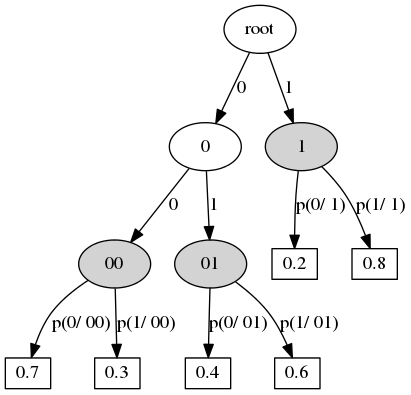
\includegraphics[scale=0.4]{img/Prune_c_trie.png}
	\centering
	\caption{ Подрезанное контекстое дерево }
	\label{ris:prune_c_trie}
\end{minipage}
\end{figure}
Можно заметить, что в этом примере, имея для некоторого состояния $x_{t}$ контекст  <<$1$>> , необходимость уточнять его (т.е. спускаться дальше к листу) отсутствует, т.к. распределение на контекстах  <<$10$>>  и  <<$11$>>  одно и тоже. 
Таким образом подрезанное дерево с рисунка \ref{ris:prune_c_trie} задает такие же распределения переходов как и дерево с рисунка \ref{ris:context_trie}. 
Однако второе контекстное дерево меньше (число главных контекстов меньше).
Но не один Марковский процесс фиксированного порядка напрямую его использовать не может.

Определим процесс, который может иметь распределение переходов в виде дерева с рисунка \ref{ris:prune_c_trie}.

Пусть $\tau$ --- конечное контекстное дерево.
Для $s \in \tau$ будем обозначать через $ C(s) $ множество всех потомков, являющихся листами $\tau$. 
Для $s \notin \tau$, $C(s)$ --- лист $\tau$, являющийся префиксом  $s$ (можно заметить, что он существует и единственен).
\begin{definition}
\textit{Марковский процесс переменного порядка} (МППП) с максимально-возможным порядком $m$ --- это вероятностный процесс, распределения на состояниях которого задаются распределниями на листьях некоторого контекстного дерева $\tau$ глубины не более чем $m+1$, и 
\[ P(q |s) =
  \begin{cases}
    P(q|C(s))       & \quad \text{для } s \notin \tau\\
    \frac{\sum_{c \in C(s)} {P(q|c)P(c)}}{\sum_{q' \in S}\sum_{c \in C(s)} {P(q'|c)P(c)}} & \quad \text{для } s \in \tau\\
  \end{cases}
\]
вероятность того, что следующее состояние за цепью $s$ является $q$
\label{def:c_trie}
\end{definition}

\begin{definition}
Марковская модель переменного порядка (ММПП) с максимально-возможным порядком $m$ --- вероятностная модель, описывающая соответствующий процесс.
Параметрами модели являются множество переходов на листьях некоторого контекстного дерева $\tau$ глубины не более чем $m+1$ и вероятностное распределение на них (листьях).
\end{definition}

\begin{remark}
МППП с максимально-возможным порядком $m$ есть обобщение всех скрытых Марковских процессов порядка меньше либо равного, чем $ m $.
\end{remark}

\subsection{Скрытые Марковские модели}
Представим, что состояния --- это какой-то скрытый признак/фактор (например, наличие или отсутствие связи белка и ДНК) цепи наблюдений $Y = \{y_{t}\}_{t \in Z_{+}}$. Для каждого наблюдения $y_{t}$ он не известен, однако именно он определяет распределение на $Y_{t}$.

Т.е. цепь $Y$ порождается из Марковской цепи $X = \{x_{t}\}_{t \in Z_{+}}$ путем покоординатного определения новой случайной величины $Y_{t}$ для каждого состояния $x_{t}$ согласно распределению $P(.|~x_{t})$.

\begin{definition}
Процесс, порождающий цепь по некоторому Марковскому процессу $X = \{x_{t}\}_{t \in Z_{+}}$ порядка $m$ и распределению $P(.|~x_{t})$, называется \textit{скрытым Марковским процессом порядка $m$}. 
$ X $ называеются \textit{скрытыми состоянияниями}, $Y$ --- \textit{наблюдениями}.
\end{definition}

\begin{definition}
\textit{Скрытая Марковская модель} (СММ) порядка $ m $ --- вероятностная модель, описывающая соответствующий процесс. Параметрами модели является $\Lambda=(A,\pi,B)$, где $A,\pi$ --- параметры скрытого процесса $X$ порядка $m$,  $ B = \{b(y; x)\}_{y \in R^{l}, x \in S}$ ---  множество распределений испусканий (где $ b(y; x) = P(y|x)$). 
\end{definition}

\begin{definition}
\textit{Скрытая Марковская модель переменного порядка} (СММПП) --- вероятностная модель, описывающая соответствующий процесс. Параметрами модели является $\Lambda=(A,\pi,B)$, где $A,\pi$ --- параметры скрытого процесса переменного порядка $X$ ,  $ B = \{b(y; x)\}_{y \in R^{l}, x \in S}$, где $ b(y; x) = P(y|x)$ ---  множество распределений испусканий. 
\end{definition}


\subsection{Обучение модели СММПП}
Задачу обучения скрытой Марковской модели переменного порядка можно сформулировать следующим образом: 
по цепи наблюдений $ Y = (y_{1}, ... y_{T}) $ найти параметры $\Lambda = (A,B,C,\pi)$ модели СММПП, которые бы минимизировали количество контекстов не сильно ухудшая правдоподобие модели по сравнению с правдоподобием модели на полном дереве (допустимое отклонение распределений регулирует параметр $ \epsilon_{\text{prune}} $).

На рисунке \ref{alg} схематично представлен алгоритм обучения СММПП. Ниже подробно описаны основные шаги: инициализация, EM, подрезание дерева.
\\

\begin{algorithm}[H]
 \KwData{
 \\$Y$,  // наблюдения
 \\$ m $, $ \epsilon_{\textit{EM}} $, $ \epsilon_{\textit{prune}} $  
 \\//параметры обучения: максимальная длина контекста, 
 \\//порог для остановки EM, порог для обрезания дерева}
 \KwResult{$\Lambda$  // параметры СММПП}
 \textit{
 $\Lambda$ = Инициализация()
 }\;
 // полное контекстное дерево\\
 \While{контекстное дерево уменьшается}{
 	\textit{
 	$\Lambda$ = EM($Y$, $\Lambda$, $ \epsilon_{\textit{EM}} $)}\; 
 	// максимизируем правдоподобие модели на наблюдениях 
 	\\//при фиксированной структуре дерева
	\\\textit{
	$\Lambda$ = Подрезание($\Lambda$, $ \epsilon_{\textit{prune}} $)}\; 
	// подрезаем дерево, если обученные распределения при этом несильно
	\\// изменяются
 }
 \caption{Схема обучения СММПП}
 \label{alg}
\end{algorithm}


\subsubsection{Инициализация}
Начальное контекстное дерево является полным глубины $m+1$ (соответствеут CMM порядка $m$).

В качестве начальных распределений переходов и параметров испусканий берутся оценки этих величин на цепи состояний, полученной алгоритмом $k$-means ($k=|S|$) по цепи наблюдений $Y$. 
Вообще, EM допускает случайную инициализацию. Выбор конкретной обуславивается выбором распределений Пуассона в качестве распределений испусканий.

\subsubsection{EM (Expectation–Maximization algorithm)}
Пересчет производится подобно алгоритму Баума-Велша для СММ \cite{Rabiner1989}.
\\
\begin{enumerate}
\item E-шаг (Expectation)
\\Дополнительный параметр $\alpha$
$$ \alpha_{t}(c) = P(y_{0}^{t}, c(x_{t})=c| \Lambda)$$
$\alpha_{t}(c)$ --- вероятность породить первые $t+1$ наблюдений равными $y_{0}^{t}$, имея главным контекстом  скрытого состояния $x_{t}$ контекст $ c $, из модели СММПП с параметрами $\Lambda$
$$ \alpha_{0}(c) = \pi(c)b(y_{0}; c)$$ 
$$ \alpha_{t+1}(c) = \sum_{q \in S, c'=C(cq)}{\alpha_{t}(c')a(c[0];c')b(y_{t+1}; c[0])}$$
\\Дополнительный параметр $\beta$
$$ \beta_{t}(c) = P(y_{t+1}^{T}| c(x_{t})=c, \Lambda))$$
$\beta_{t}(c)$ --- вероятность того, что последние $T-t$ наблюдений цепи длины $T$, порожденной из модели СММПП с параметрами $\Lambda$, в которой главный контекст скрытого состояния $x_{t}$ является $ c $, совпадают с $y_{t+1}^{T}$
$$ \beta_{T}(c) = 1$$ 
$$ \beta_{t}(c) = \sum_{q \in S, c'=C(qc)}{a(q;c)b(y_{t+1}, c'[0])\beta_{t+1}(c')}$$
\\Дополнительный параметр $\gamma$
$$ \gamma_{t}(c) = P(x_{t}=c|Y,\Lambda) $$ 
$\gamma_{t}(c)$ --- вероятность того, что породив цепь $Y$ моделью СММПП c параметрами $\Lambda$,
главный контекст скрытого состояния $ x_{t} $ является $c$;
$$ \gamma_{t}(c) \propto {\alpha_{t}(c)\beta_{t}(c)}$$

\item M-шаг (Maximization)\\
На этом шаге алгоритм обновляет параметры модели, максимизируя правдоподобие при условии посчитанных $\alpha, \beta, \gamma$.

Для пересчета параметра $A$ вводится параметр $\xi$
\begin{align*}
\xi_{t}(q;c) = P(c(x_{t})=c, x_{t+1} = q| Y, \Lambda)
\end{align*}
$\xi_{t}(q;c)$ --- вероятность того, что породив цепь $Y$ моделью СММПП c параметрами $\Lambda$, 
главный контекст скрытого состояния $ x_{t} $ является $c$ и состояние $ x_{t+1} $ совпадает с $q$
\begin{align*}
\xi_{t}(q;c) \propto {\alpha_{t}(c)a(q;c)b(y_{t+1},q)\beta_{t+1}(qc)} 
\end{align*}
Обновление $ A $ по $ \xi $\\
$$ a(q; c) = \frac{\sum_{t}\xi_{t}(q,c)}{p(c)}$$
где $p(c) \propto \sum_{t}\gamma_{t}(c)$

Пересчет $ B $ зависит от принятого семейства моделей испусканий и производится с помощью $ \gamma $ в точности также, как и в алгоритме Баума-Велша.
В случае распределения Пуассона
$b(.~|~c) \sim \textit{Poisson}(\lambda_{c})$ 
пересчет параметров происходит следующим образом:
$$ \lambda_{c} = \frac{\sum_{t}{\gamma_{t}(c)y_{t}}}{\sum_{t}{\gamma_{t}(c)}}$$
\end{enumerate}
EM-алгоритм запускает поочередно E-шаг и M-шаг, пока правдоподобие с предыдущей итерации отличается от правдоподобия с текущей итерации более, чем на $ \epsilon_{\textit{EM}}$, т.е. пока итерация дает значимый прирост правдоподобия
$$P(Y| \Lambda) = \sum_{c \in C}\alpha_{T}(c)$$

\begin{remark} При пересчете вероятности могут очень близко подходить к нулю, что отрицательно влияет на точность расчета. Для избежания этой проблемы все расчеты проводятся не с вероятностями, а с их логарифмами.
\end{remark}

\begin{remark} EM-алгоритм следует запускать несколько раз, т.к. он может <<застревать>> в локальных максимумах функции правдоподобия.
\end{remark}

\subsubsection{Подрезание дерева} 
Если существует внутренний лист контекстного дерева $ s $ такой, что 
$$ \forall q \in S \;\; P(sq)\textit{KL}(sq, s) < \epsilon_{\textit{prune}} $$
(дети не уточняют родителя), то $ s $ становится листом, а все его потомки обрезаются, где
\begin{align*}
\textit{KL}(u, w) = \sum_{q' \in S} P(q'|u) log\frac{P(q'|u)}{P(q'|w)}
\end{align*}
расстояния Кульбака-Лейблера для апостериорных распределений.
\\Если таких листьев не существует, алгоритм заканчивает работу.

Пересчет параметров $ A $, $\pi$ на новых контекстах:
$$a_(q; c_{\textit{new}}) = P(q| c_{\textit{new}})$$
пересчитывается по определению [\ref{def:c_trie}] контекстного дерева
\begin{align*}
p_(c_{\textit{new}}) = \sum_{c \in C(c_{\textit{new}})}{p(c)}
\end{align*}


\subsection{Обучение на нескольких выборках}
В случае пропусков в наблюдениях (связанных, например, с отсутствием данных), обучение модели может проходить на множестве из нескольких цельных кусков наблюдений.
Т.е. на вход алгоритма будет подаваться не одна выборка $Y$, а                                                                                                                                                                                                                                                                                                                                                                                                                                                                                                                                                                                                                                                              $ N $ выборок $ \{Y^{1} \ldots Y^{N}\}$, подчиненных единому скрытому Марковском процессу переменного порядка.

Для применения вышеописанного алгоритма для обучения СММПП на нескольких выборках были внесены изменения в E-шаг и M-шаг.
\\
\begin{enumerate}
\item E-шаг\\
Дополнительные параметры $\alpha^{d}, \beta^{d}, \gamma^{d}, \xi^{d}$ пересчитываются отдельно по каждой выборке $d \in {1, \ldots, N}$
\\
Общая $\gamma$ - конкатенация гамм на выборках
$$ \gamma = [\gamma^{1}, \ldots ,\gamma^{N}] $$
$$ p = \prod_{d}{p^{d}}$$
\item M-шаг\\
$$ a(q; c) \propto \frac{\sum_{d}{\sum_{t}{\xi^{d}_{t}(q;c)}}}{\sum_{t}{\gamma_{t}(c)}} $$
$$P(\{Y^{1} \ldots Y^{N}\}|\Lambda) = \prod_{d}{P(Y^{d}|\Lambda)}$$
\end{enumerate}

\subsection{Сравнение}
Чем больше параметров у модели, тем лучше она подстраивается под данные, и тем проще переобучается. 
Поэтому, при сравнении моделей, обученных на одних и тех же данных, со схожим правдоподобием, предпочтительней будет та, которая проще. 
Конкретную величину, которую следует сравнивать для моделей, обученных на одинаковых данных, предлагает критерий Акаике (AIC)
$$ AIC = 2k-2\log{L} $$ 
где $ k $ --- число степеней свободы или число параметров модели, $ L $ --- максимальное правдоподобие модели на заданной выборке. Чем $AIC$ меньше, тем модель лучше. 

Число параметров для СММПП с $ n $ скрытыми состояниями, $ l $ контекстами, и Пуассоновскими испусканиями 
\begin{align*}
k &= [\text{количество степеней свободы} \; A ] 
+ [\text{количество степеней свободы} \; B ]
\\&+ [\text{количество степеней свободы} \; \pi ]
\\ &= l(n-1)\;+\;n\;+\;(l-1) \\&= nl + n - 1
\\
\text{При } n=2, k &= 2l + 1
\end{align*}

Для СММ порядка $m$, $l=2^m$, поэтому $k = 2^{m+1}+1$

\section{Реализация}
Общий алгоритм обучения скрытой Марковской модели переменного порядка был реализован на языке программирования Python. 

Критическим по производительности является E-шаг, он был перенесен на Cython.

Основные использованные библиотеки.
\begin{itemize}
\item
NumPy, SciPy для операций над матрицами.
\item
Joblib для распараллеливания по потокам.
\\
В случае обучения на нескольких выборках, E-шаг для каждой выборки считается независимо, по этому эту часть можно параллелить.
\item
Pygraphviz для отрисовки деревьев. 
\item
Matplotlib для отрисовки графиков.
\end{itemize}

\section{Применение}
\subsection{Применение к симмулированным данным}
Проверка работы алгоритма обучения происходила следующим образом:
\begin{enumerate}
\item
генерировались параметры $\Lambda$ начальной модели СММПП;
\item
порождались несколько выборок $ Y $ из заданной модели;
\item
находились новые параметры $\hat{\Lambda}$ путем обучения модели на порожденных выборках;
\item
сравнивались полученные параметры $\hat{\Lambda}$ с реальными $\Lambda$,
считалось абсолютное среднее отклонение параметров реальной модели от предсказанных параметров. 
\end{enumerate}

Ниже проиллюстрирована работа алгоритма на простых моделях: Пуассоновская смесь (СММ нулевого порядка) и СММ (СММ первого порядка). Также проиллюстрирован более интересный случай: СММПП, не являющейся СММ фиксированного порядка.

Для каждого теста было сгенерировано по $100$ выборок длиной $5000$.
Значения параметров алгоритма обучения были выбраны следующими: максимально-возможный порядок $m=4$, порог для обрезания $ \epsilon_{\textit{prune}} = 0.007$, порог для остановки EM $\epsilon_{\textit{EM}} =  0.01 $ 

Были посчитаны абсолютное среднее отклонение (MAE --- Mean Absolute Error) полученных распределений переходов от реальных распределений, отклонение параметров Пуассоновского испускания $\lambda$ от реальных, оценка математического ожидания доли ложных единиц среди всех предсказанных единиц $\hat{\textit{fdr}}$ (false discovery rate), оценка математического ожидания доли ложных нулей среди всех предсказанных нулей $\hat{\textit{fndr}}$ (false nondiscovery rate).
Среднее значение, полученное обучением модели на разных выборках при фиксированой начальной модели, этих величин показаны в соответствующих таблицах.

\subsubsection{Пуассоновская смесь}
Модель смеси была выбрана с параметрами переходов, изображенных контекстным деревом на рисунке \ref{ris:sample_mixture_real_trie}, параметрами испусканий
$$B = \{\textit{Poisson}(\lambda=2), \textit{Poisson}(\lambda=10)\}$$.

Сравнение полученных в ходе обучения параметров с реальными, $\hat{\textit{fdr}}$, $\hat{\textit{fndr}}$ показаны в таблице \ref{table_mixture}.
\begin{center}
    \begin{tabular}{ |l|*{4}{m{2cm}|} }
     \hline
     & $\textit{MAE}(A, \hat{A})$ & $\textit{MAE}(\lambda, \hat{\lambda})$ & $\hat{\textit{fdr}}$ & $\hat{\textit{fndr}}$
     \\ \hline
     $\textit{Среднее по тестам}$ & $0.07$ & $0.21$ & $0.01$ & $0.02$
     \\ \hline
    \end{tabular}
    \label{table_mixture}
\end{center}
Пример предсказанного дерева изображен на рисунке \ref{ris:sample_mixture_predicted_trie}.
\begin{figure}[h!]\centering
\begin{minipage}[b]{0.49 \textwidth}
	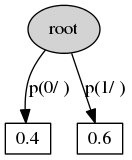
\includegraphics[scale=0.57]{img/sample_mixture/real_trie_.png}
	\centering
	\caption{ Реальное дерево }
	\label{ris:sample_mixture_real_trie}
	
\end{minipage}
\hfil \hfil%раздвигаем боксы по горизонтали
\begin{minipage}[b]{0.49 \textwidth}
	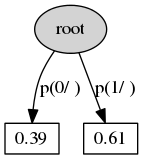
\includegraphics[scale=0.57]{img/sample_mixture/predicted_trie.png}
	\centering
	\caption{ Предсказанное дерево }
	\label{ris:sample_mixture_predicted_trie}
\end{minipage}
\end{figure}

\subsubsection{СММ}
Модель СММ была выбрана с параметрами переходов, изображенных контекстным деревом на рисунке \ref{ris:sample_hmm1_real_trie}, параметрами испусканий
$$B = \{\textit{Poisson}(\lambda=1), \textit{Poisson}(\lambda=8)\}$$.

Сравнение полученных в ходе обучения параметров с реальными, $\hat{\textit{fdr}}$, $\hat{\textit{fndr}}$ показаны в таблице \ref{table_hmm1}.
\begin{center}
    \begin{tabular}{ |l|*{4}{m{2cm}|} }
     \hline
     & $\textit{MAE}(A, \hat{A})$ & $\textit{MAE}(\lambda, \hat{\lambda})$ & $\hat{\textit{fdr}}$ & $\hat{\textit{fndr}}$
     \\ \hline
     $\textit{Среднее по тестам}$ & $0.09$ & $0.21$ & $0.02$ & $0.02$
     \\ \hline
    \end{tabular}
    \label{table_hmm1}
\end{center}
Пример предсказанного дерева изображен на рисунке \ref{ris:sample_hmm1_predicted_trie}.

На рисунке \ref{ris:sample_hmm1_log_likelihood} изображен график обучения. Каждая EM-часть выделена боксом, сверху которого написано число контекстов на момент обучения, снизу количество итераций в этой части и параметры распределения испусканий, полученных на последней итерации, внутри --- график логарифма правдоподобия по итерациям EM. 
На такой схеме видно, как сначала алгоритм 6 итераций EM обучался на 16 контекстах, после чего дерево подрезалось до 2 контекстов. Следующему EM не удалось значимо увеличить правдоподобие модели, поэтому на третей итерации он закончил работу. Далее дерево не удалось еще раз подрезать, поэтому весь алгоритм закончил свою работу (это видно из отсутствия следующего бокса под график ЕM).
\begin{figure}[h!]\centering
\begin{minipage}[b]{0.49 \textwidth}
	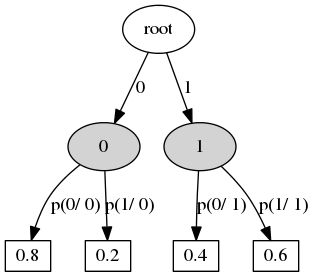
\includegraphics[scale=0.4]{img/sample_hmm1/real_trie_.png}
	\centering
	\caption{ Реальное дерево }
	\label{ris:sample_hmm1_real_trie}
\end{minipage}
\hfil \hfil%раздвигаем боксы по горизонтали
\begin{minipage}[b]{0.49 \textwidth}
	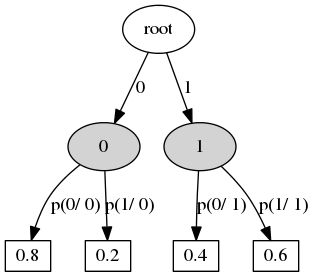
\includegraphics[scale=0.4]{img/sample_hmm1/predicted_trie.png}
	\centering
	\caption{ Предсказанное дерево }
	\label{ris:sample_hmm1_predicted_trie}
\end{minipage}
\begin{minipage}[b]{0.8 \textwidth}
	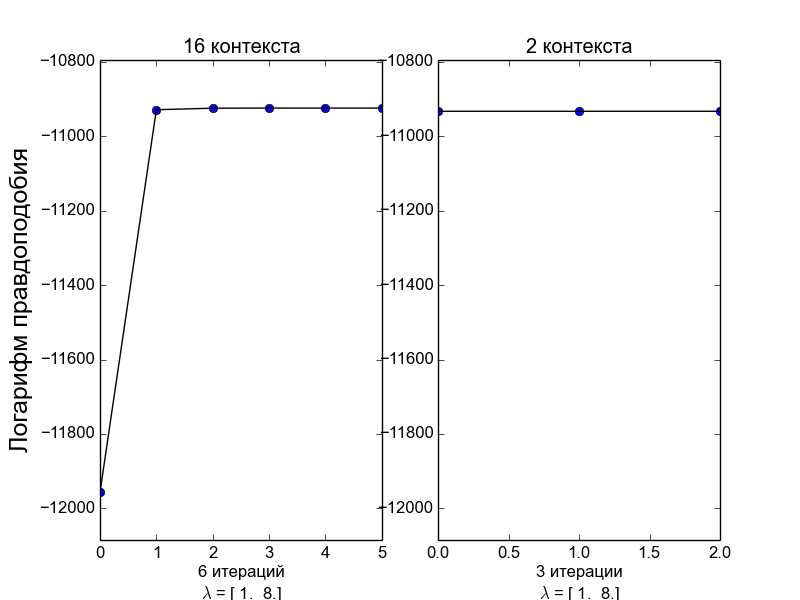
\includegraphics[scale=0.4]{img/sample_hmm1/plot_.png}
	\centering
	\caption{ График обучения }
	\label{ris:sample_hmm1_log_likelihood}
\end{minipage}
\end{figure}

\subsubsection{Более интересный случай, СММПП}
Модель СММПП была выбрана с параметрами переходов, изображенных контекстным деревом на рисунке \ref{ris:sample_vlhmm_real_trie}, параметрами испусканий
$$B = \{\textit{Poisson}(\lambda=3), \textit{Poisson}(\lambda=15)\}$$.

Сравнение полученных в ходе обучения параметров с реальными,$\hat{\textit{fdr}}$, $\hat{\textit{fndr}}$ показаны в таблице \ref{table_vlhmm}.
\begin{center}
    \begin{tabular}{ |l|*{4}{m{2cm}|} }
     \hline
     & $\textit{MAE}(A, \hat{A})$ & $\textit{MAE}(\lambda, \hat{\lambda})$ & $\hat{\textit{fdr}}$ & $\hat{\textit{fndr}}$
     \\ \hline
     $\textit{Среднее по тестам}$ & $0.11$ & $0.20$ & $0.02$ &  $0.02$
     \\ \hline
    \end{tabular}
    \label{table_vlhmm}
\end{center}
Пример предсказанного дерева изображен на рисунке \ref{ris:sample_vlhmm_predicted_trie}.

На рисунке \ref{ris:sample_vlhmm_log_likelihood} представлен график обучения модели на одном из тестов.

\begin{figure}[h!]\centering
\begin{minipage}[b]{0.49 \textwidth}
	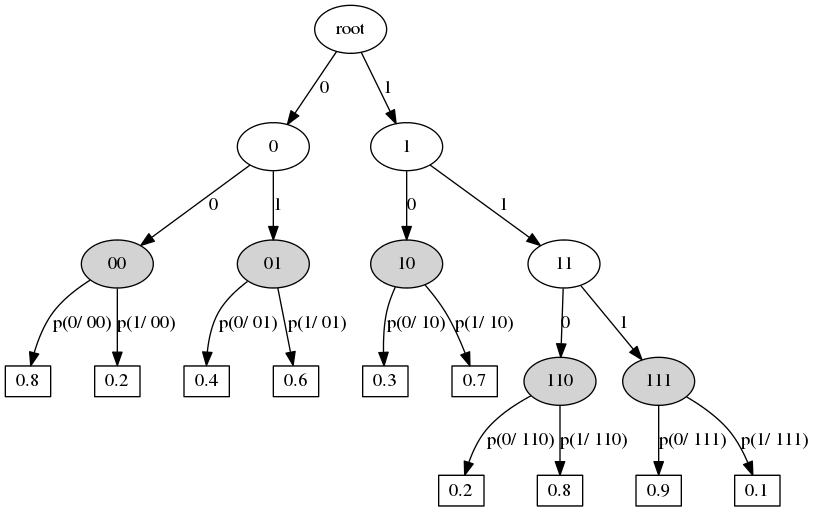
\includegraphics[scale=0.3]{img/sample/real_trie_.png}
	\centering
	\caption{ Реальное дерево }
	\label{ris:sample_vlhmm_real_trie}
	
\end{minipage}
\hfil \hfil%раздвигаем боксы по горизонтали
\begin{minipage}[b]{0.49 \textwidth}
	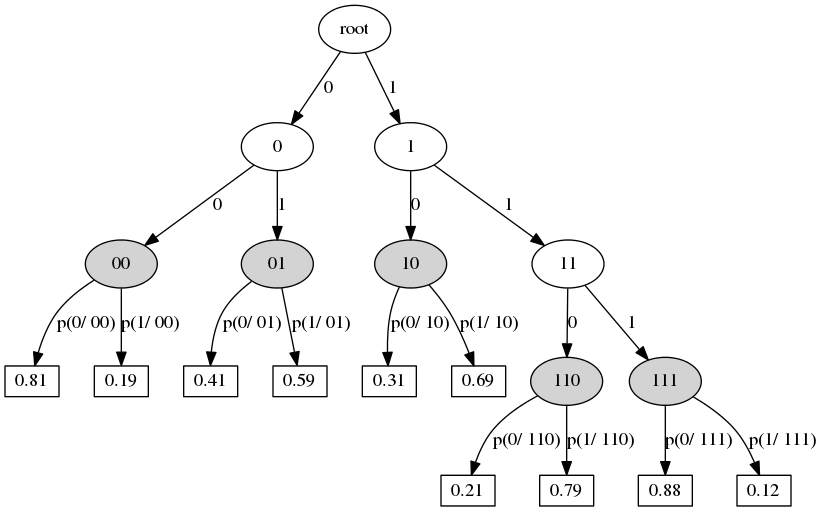
\includegraphics[scale=0.3]{img/sample/predicted_trie.png}
	\centering
	\caption{ Предсказанное дерево }
	\label{ris:sample_vlhmm_predicted_trie}
\end{minipage}
\begin{minipage}[b]{0.8 \textwidth}
	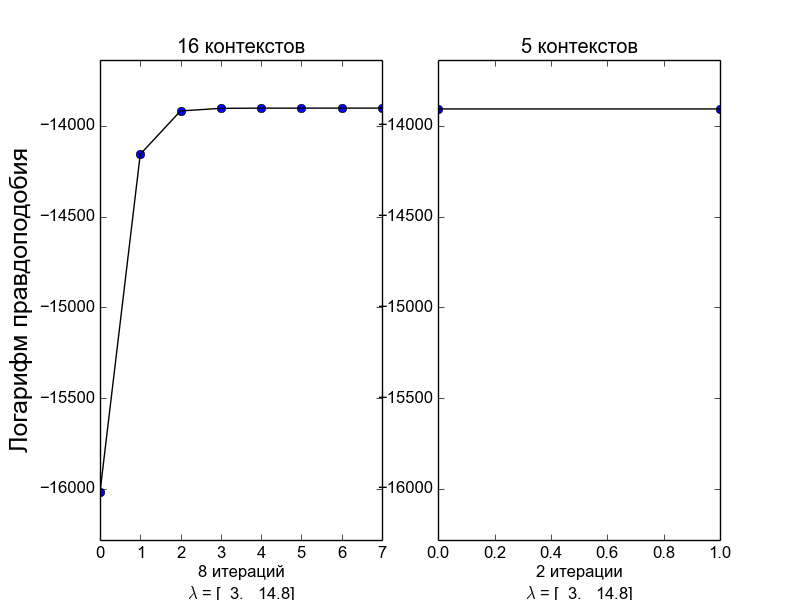
\includegraphics[scale=0.4]{img/sample/plot_.png}
	\centering
	\caption{ График обучения }
	\label{ris:sample_vlhmm_log_likelihood}
\end{minipage}
\end{figure}

\subsection{Применение к реальным данным}
Данные были взяты из проекта ENCODE (ENCyclopedia of DNA Elements).
В качестве исследуемого белка был выбран гистон H3 с ацетилированным лизином в 27-й позиции. Рассматриваемые клетки --- эмбриональные стволовые клетки человека \cite{ENCODE}.
Размер окна был выбран равный 200 п.н.

В качестве выборок были рассмотрены ненулевые участки массива, полученного после деления результата эксперимента ChIP-seq на окна.  

Ниже приведены результаты обучения на данных четвертой хромосомы (размер полученной выборки $\sim 10^5$)

Параметры обучения были выбраны следующими:
$m = 5$, $\epsilon_{\textit{prune}} = 0.04$, $\epsilon_{\textit{em}} = 0.05$

График обучение изображен на рисунке \ref{ris:log_likelihood}.
Из него видно, как сначала алгоритм 12 итераций EM обучался на 32 контекстах, потом подрезал дерево до 5 контекстов. После чего ни обучение, ни подрезание не дало результатов, поэтому, алгоритм закончил работу.

Полученное контекстное дерево переходов для скрытого слоя состояний, отвечающих за ДНК-белковую связь проиллюстрировано на рисунке \ref{ris:real_trie}. Из него видно каким образом наличие взаимодействия с белком в фиксированном окне генома определяется взаимодействиями в предшествующих окнах.

\begin{figure}[h!]\centering
\begin{minipage}[b]{0.49 \textwidth}
	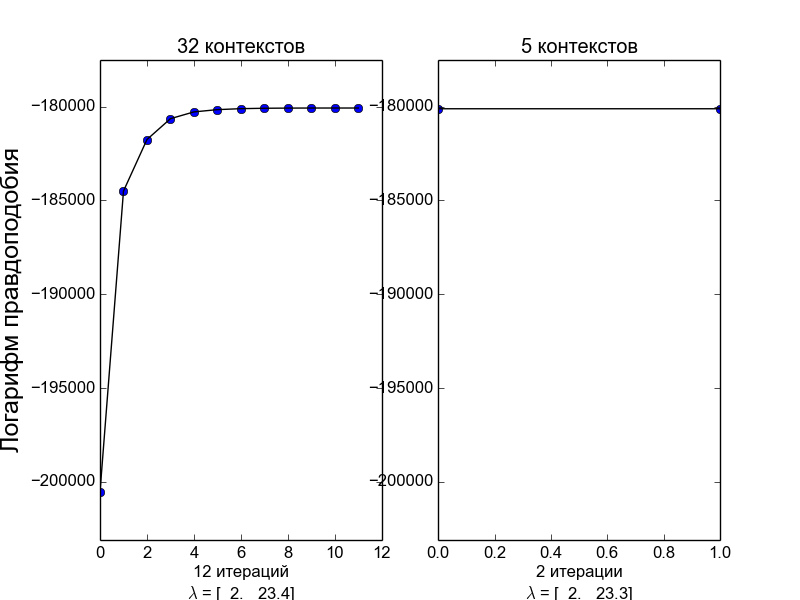
\includegraphics[scale=0.47]{img/real/plot_.png}
	\centering
	\caption{ График обучения }
	\label{ris:log_likelihood}
\end{minipage}
\hfill
\begin{minipage}[b]{0.32 \textwidth}
	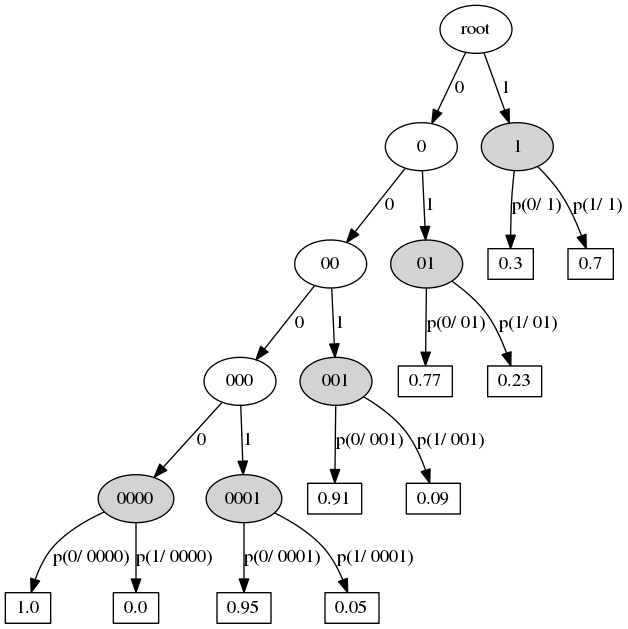
\includegraphics[scale=0.29]{img/real/predicted_trie.png}
	\centering
	\caption{ Контекстноe дерево }
	\label{ris:real_trie}
\end{minipage}
\end{figure}

Ниже представлено сравнение логарифма правдоподобия \ref{ris:real_comp_log_p}, критерия Акаике \ref{ris:real_comp_aic} и времени обучения \ref{ris:real_comp_time} для моделей СММПП, СММ5 (СММ 5-го порядка, соответствует дереву, с которого начиналось обучение СММПП) и СММ (СММ 1-го порядка, именно его чаще всего используют для анализа данных ChIP-seq).
\begin{figure}[h!]\centering
\begin{minipage}[b]{0.32 \textwidth}
	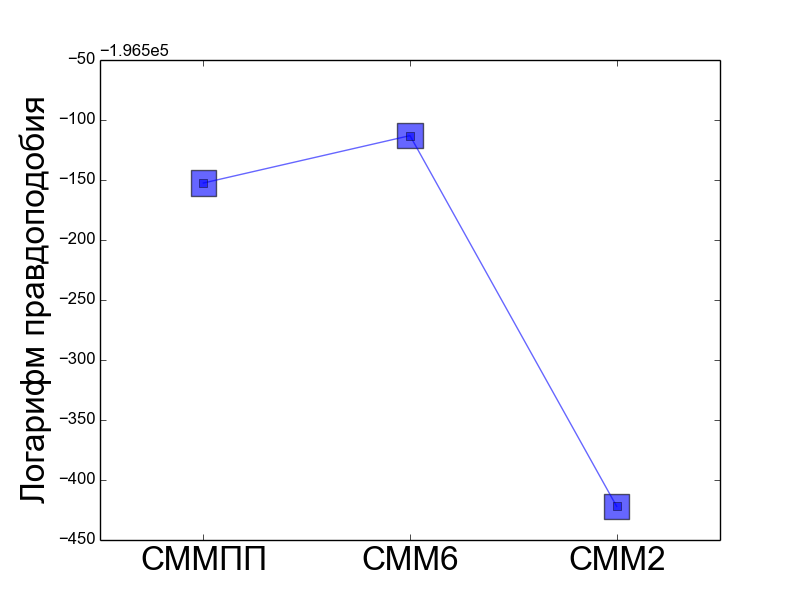
\includegraphics[scale=0.28]{img/real/log_p.png}
	\centering
	\caption{ Сравнение логарифма правдоподобия}
	\label{ris:real_comp_log_p}
\end{minipage}
\hfill
\begin{minipage}[b]{0.32 \textwidth}
	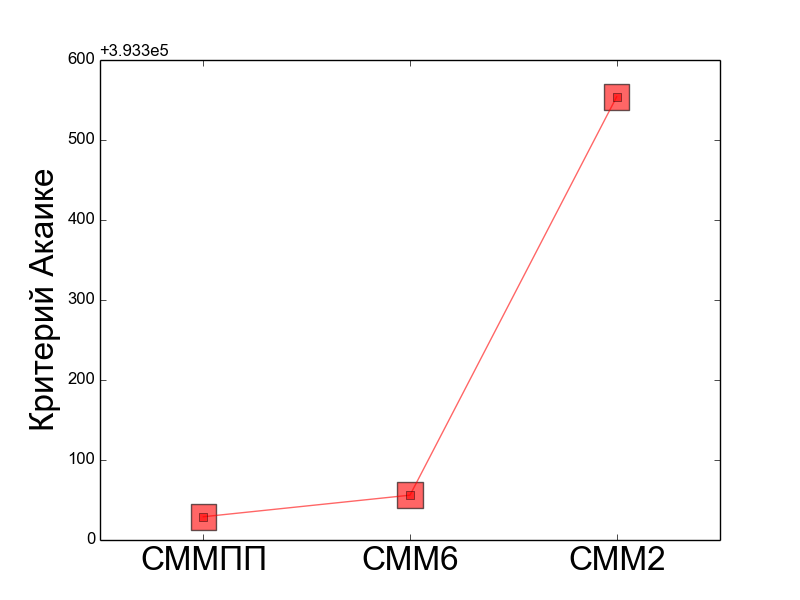
\includegraphics[scale=0.28]{img/real/aic.png}
	\centering
	\caption{ Сравнение критерия Акаике }
	\label{ris:real_comp_aic}
\end{minipage}
\hfill
\begin{minipage}[b]{0.32 \textwidth}
	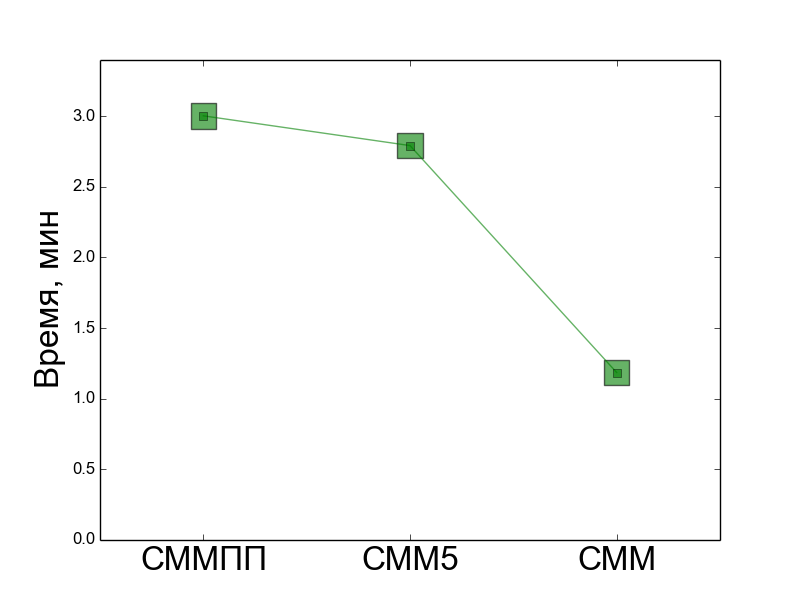
\includegraphics[scale=0.28]{img/real/time.png}
	\centering
	\caption{ Сравнение времени обучения }
	\label{ris:real_comp_time}
\end{minipage}
\end{figure}

По критерию Акакике выигрывает СММПП (напомним, что данный критерий, чем меньше, тем лучше).

СММ5 имеет лучшее среди этих трех моделей правдоподобие, однако ее губит большое количество параметров. 
СММ имеет меньшее среди данных моделей количество параметров, однако ее правдоподобие совсем невелико.

Рисунок \ref{ris:real_trie} показывает сравнение времени обучения. Тут СММПП дает похожий результат с СММ5, немного ей уступая. СММ, в силу того, что она имеет более простую структуру, обучается быстрее всех.


\section*{Заключение}
В ходе работы были решены поставленные задачи:
\begin{enumerate}
\item
реализована СММПП, подходящая под данные ChIP-seq;
\item
проведен анализ эффективности работы СММППна
синтетических данных; 
\item
осуществлено применение СММПП к
данным ChIP-seq, проведено сравнение СММПП на реальных данных с более простыми моделями (СММ первого порядка, пятого);
\end{enumerate}




\bibliographystyle{plain}
\bibliography{diploma.bib}
\end{document}
